
\documentclass[letterpaper,12pt]{article}
\usepackage{tabularx} 
\usepackage{amsmath}  
\usepackage{amsthm}
\usepackage{amsfonts}
\usepackage{graphicx} 
\usepackage[margin=1in,letterpaper]{geometry} 
\usepackage{cite} 
\usepackage{graphicx} 
\usepackage[spanish]{babel}
\usepackage[export]{adjustbox}
\usepackage{wrapfig}
\usepackage[final]{hyperref} 
\usepackage[utf8]{inputenc}
\usepackage{float}
\usepackage{helvet}
\usepackage{pdfpages}
\renewcommand{\familydefault}{\sfdefault}
\hypersetup{
	colorlinks=true,      
	linkcolor=blue,       
	citecolor=blue,       
	filecolor=magenta,    
	urlcolor=blue         
}
\graphicspath{ {d:/proyectos/universidad/LaHoraDelCodigo/Planificacion/} }



\title{Propuesta de Organización para el Evento \\ \texttt{\textbf{HoraDelCódigo}} }
\author{Gonzalo Fernández C. \\ \texttt{gonzalo.fernandezc@sansano.usm.cl} }
\date{\today\\Revisión 1.0}

\usepackage{titling}
\setlength{\droptitle}{0.6in}
 
\begin{document}

\begin{titlepage}

\begin{figure}

\includegraphics[width=0.4\linewidth]{logou} 
\hspace{\fill}

\includegraphics[width=0.08\linewidth]{logo} 
\end{figure}

\maketitle

\end{titlepage}


\section{Historial de Cambios}

\begin{center}
\begin{tabular}{|c|c|c|c|}
\hline
Versión & Fecha & Autor & Comentario \\
\hline \hline
1.0 & 17/01/2018 & Gonzalo F. & Primera versión del documento \\ \hline
\end{tabular}
\end{center}

\section{Introducción}

El presente documento pretende formalizar una propuesta de organización con el fin de realizar una \texttt{\textbf{HoraDelCódigo}} en la \texttt{Universidad Técnica Federico Santa María - Campus San Joaquín}. Esta propuesta tratará temas relacionados con los tutores, participantes, los procesos de inscripción e invitación, tiempos, actividades, costos, recursos necesarios, entre otros. Al no ser esta una propuesta definitiva, el documento está abierto a modificaciones posteriores con el fin de lograr organizar de mejor forma la realización de este evento.

\section{Tutores}

Los siguientes alumnos se han ofrecido voluntariamente a participar como tutores en esta actividad guiándo a los asistentes en la realización de alguno de los talleres ofrecidos por \texttt{\textbf{HoraDelCódigo}}:

\begin{itemize}
    \item Gonzalo Fernández C. -- \texttt{gonzalo.fernandezc@sansano.usm.cl} 
    \item Martin Crisostomo B. -- \texttt{martin.crisostomo@sansano.usm.cl} 
    \item Fabian Riquelme M. -- \texttt{fabian.riquelme@sansano.usm.cl}
    \item Sebastián Alvarado A. -- \texttt{sebastian.alvaradoa@sansano.usm.cl}
    \item Christian Muñoz I. -- \texttt{christian.munozi@sansano.usm.cl}
\end{itemize}

El ideal para la realización de estas actividades es contar con la participación de a lo más 2 tutores por actividad, por lo tanto, es importante invitar a más personas ya sean estos alumnos o profesores interesados en guiar a los participantes, para esto, se ha puesto a disposición un \texttt{\href{https://goo.gl/forms/qtJc6NDwXBY16QoZ2}{Google Form}} desde el cual es posible postular.

\section{Inscripción}

El proceso de inscripción por parte de los participantes por el momento queda pendiente pues será necesario el apoyo del área de Admisión de la Universidad ya que manejan más información sobre este tipo de procesos.

\section{Horarios}

Dado que por el momento el evento está en proceso de organización, no hay una fecha definida para la realización de este, por lo tanto, en esta primera propuesta se definirá la duración de las actividades del mismo.


\begin{center}
\begin{tabular}{|c|c| p{11cm} |}
\hline
Actividad & Duración & Comentario \\
\hline \hline
Preparación & 9:30 -- 10:00 & Llegada de los Tutores y gente encargada de organizar el evento para preparar todo. \\ \hline
Acreditación & 10:00 -- 10:30 & Llegada de los participantes, presentación del evento, \emph{*entrega de poleras y stickers}, etc. (temas necesarios antes de iniciar la actividad) \\ \hline
\texttt{HoraDelCódigo} & 10:30 -- 12:30 & Comienzan las actividades del evento en los respectivos laboratorios. \\ \hline
Almuerzo & 12:30 -- 13:30 & Almorzar, se podría incluír alguna actividad para presentar la universidad. \\ \hline
Despedida & 13:30 & \emph{*Entrega de diplomas}, se terminan las actividades. \\ \hline
\end{tabular}
\end{center}

*Temas a tratar más adelante.

\section{Actividades}

Las actividades a realizar en los laboratorios durante la \texttt{HoraDelCódigo} serán elegidas desde el \texttt{\href{https://hourofcode.com/es/learn}{Sitio Oficial}} por parte de los Tutores. En esta sección se dispondrá de una lista indicando el tutor, la actividad y el laboratorio asignado para el desarrollo de esta una vez esté esta información.

\begin{figure}[H]
  \centering
    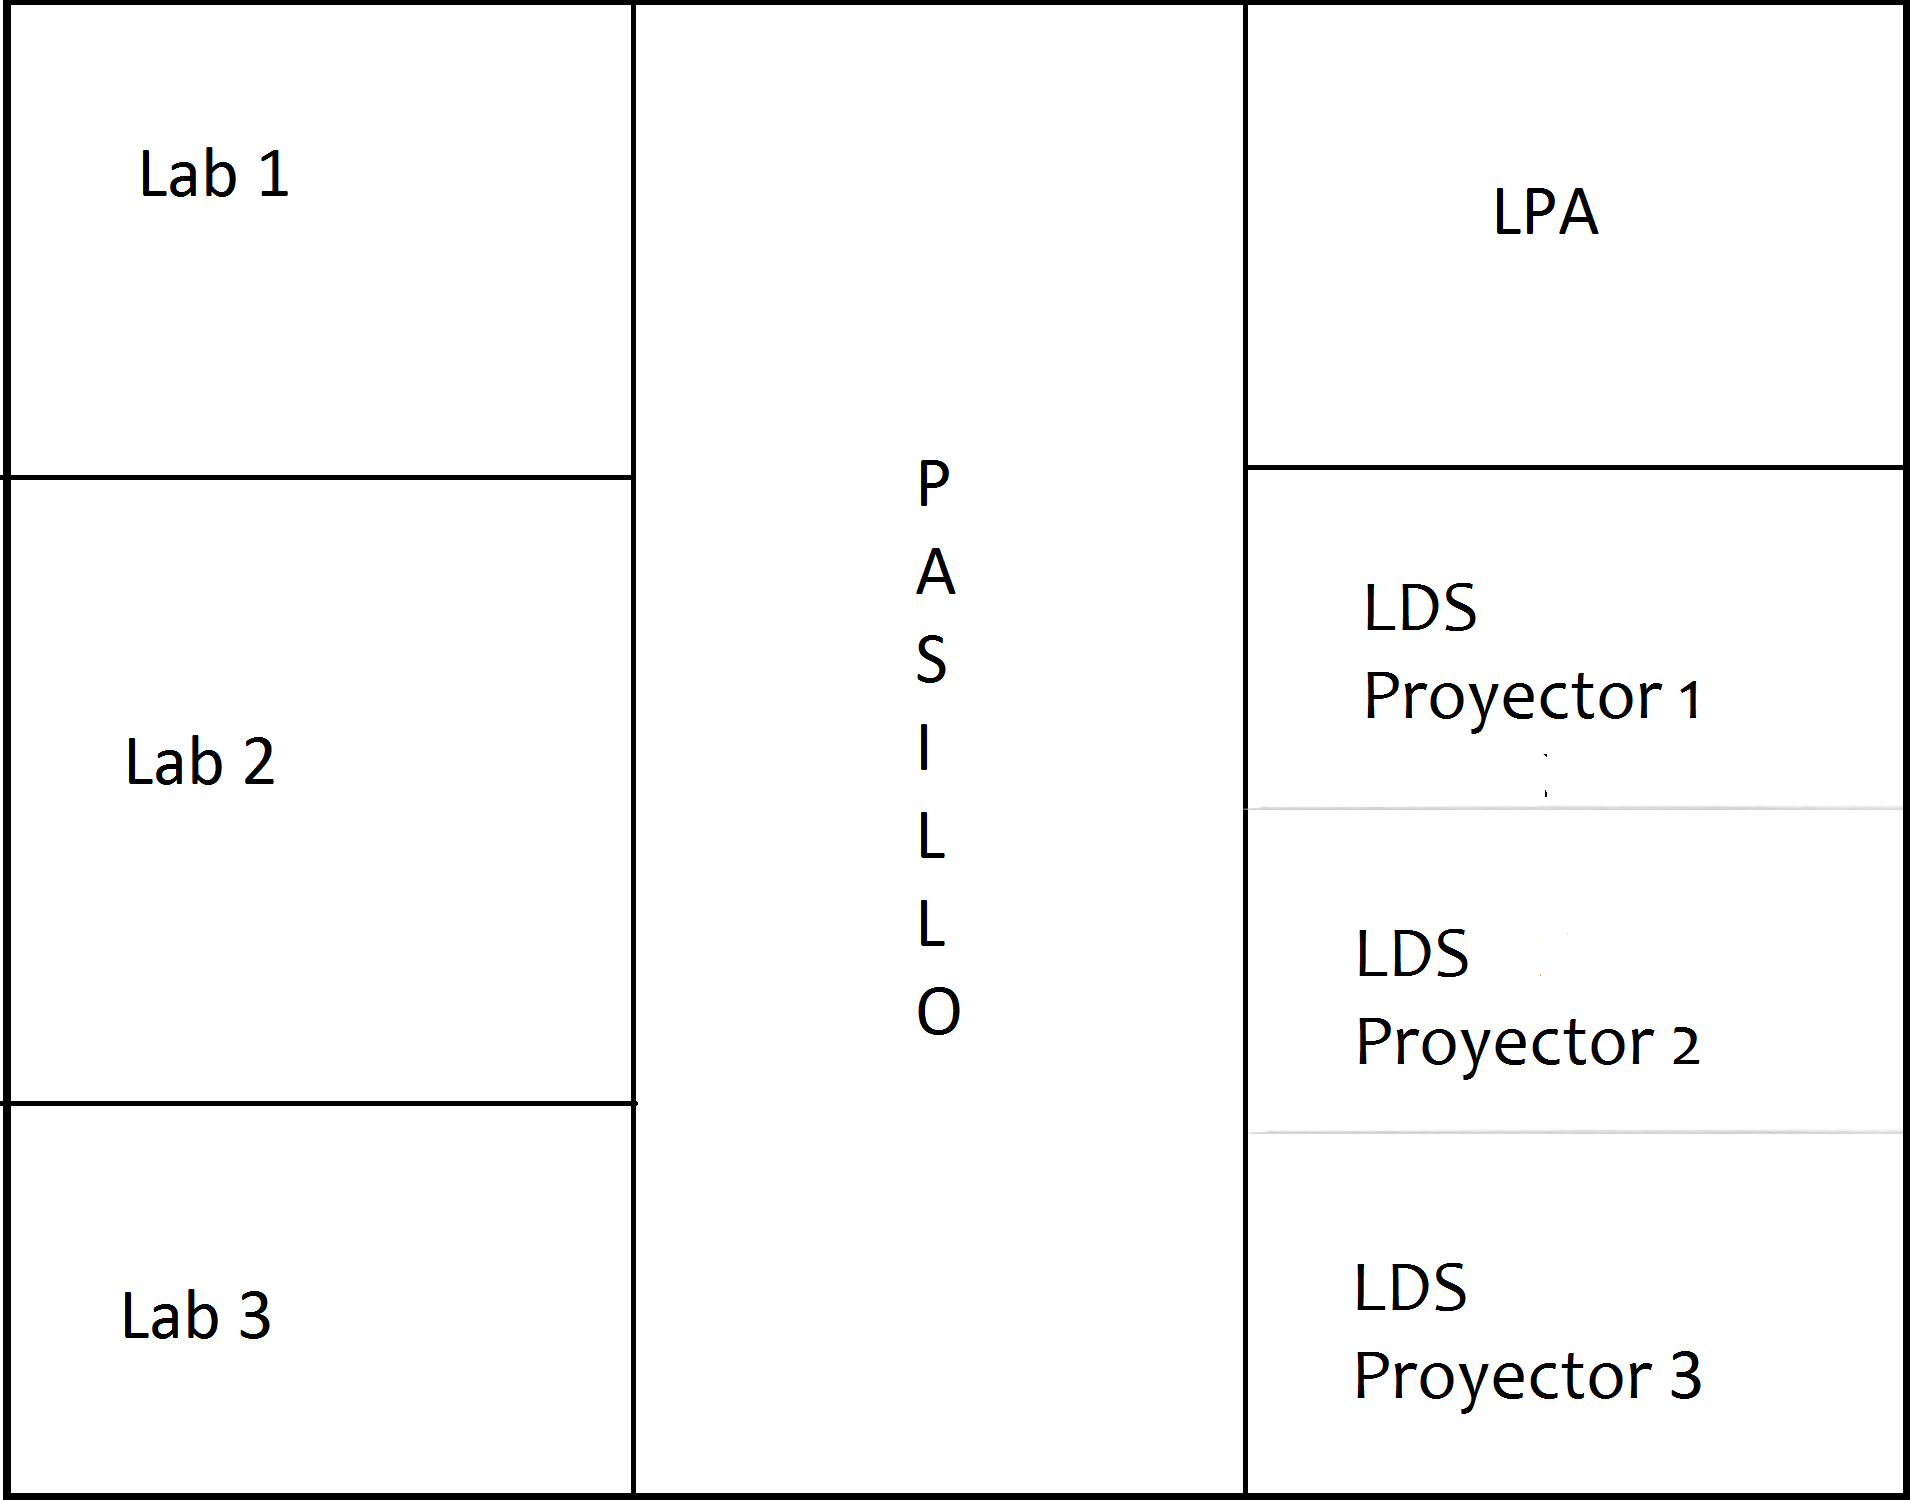
\includegraphics[width=0.6\textwidth]{salas}
  \caption{Distribución de los laboratorios para el evento.}
\end{figure}

\section{Costos}

El evento en sí no requiere de costos más allá del uso de los laboratorios antes mencionados, a excepción del almuerzo para los participantes en caso de acceder a costearlo, la siguiente lista muestra algunos items usados al momento de realizar una \texttt{HoraDelCódigo} para regalar a los participantes.


\subsection{Certificados}

Impresión de \texttt{\href{https://code.org/certificates}{Diplomas Oficiales}} para cada uno de los participantes: \$???.

\begin{figure}[H]
  \centering
    
\includegraphics[width=0.5\textwidth]{diploma}
  \caption{Certificado por completar una HoraDelCódigo .}
\end{figure}

\subsection{Poleras}

\texttt{\href{https://store.code.org/collections/all?page=2}{Poleras Oficiales}} para cada uno de los participantes: \$???

\begin{figure}[H]
  \centering
    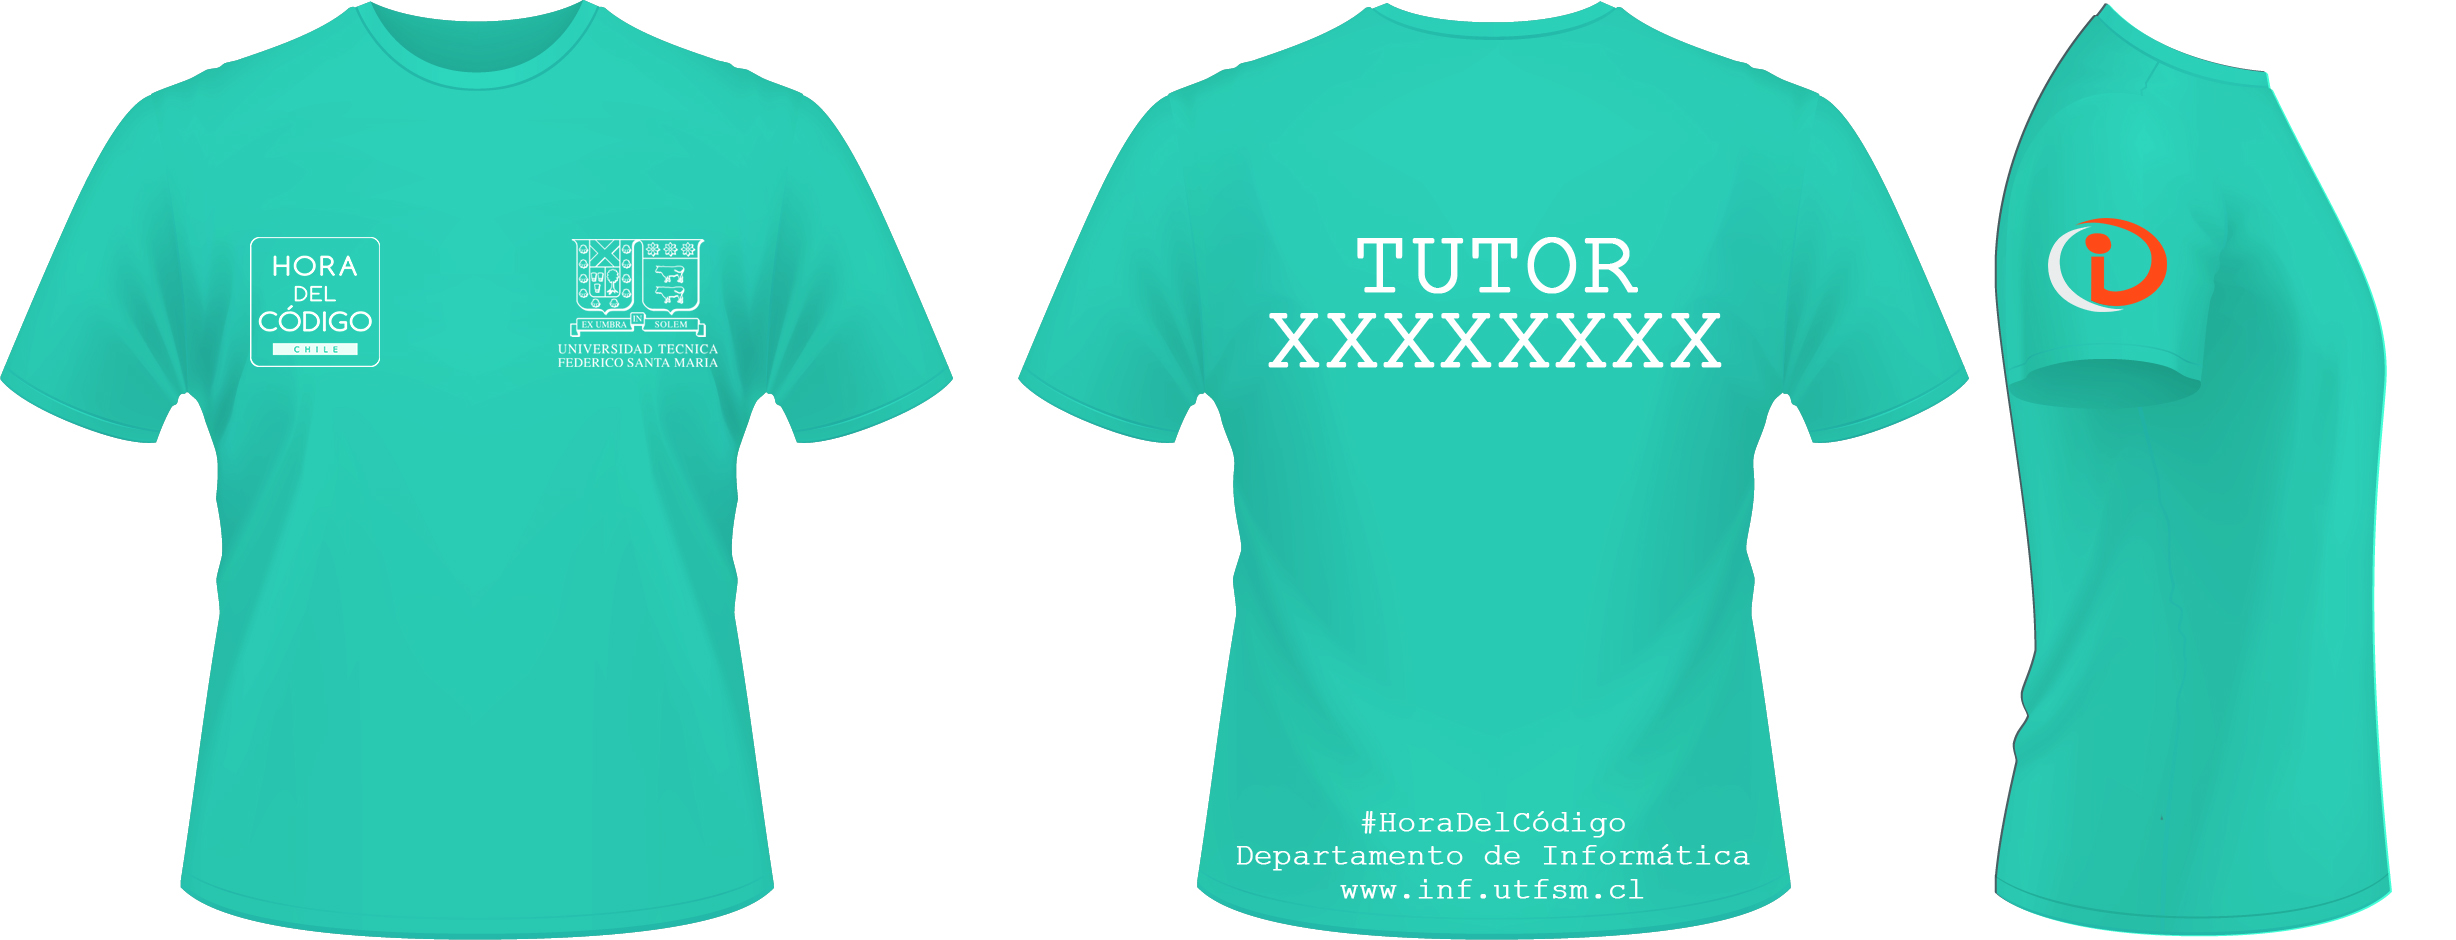
\includegraphics[width=0.5\textwidth]{poleras}
  \caption{Poleras Oficiales de la HoraDelCódigo.}
\end{figure}

\subsection{Stickers}

Impresión de stickers para cada uno de los participantes, ya sea el logo de \texttt{LaHoraDelCódigo} ó el sticket de ``Yo hice la HoraDelCódigo'': \$???

\begin{figure}[H]
  \centering
    
\includegraphics[width=0.5\textwidth]{sticker}
  \caption{Stickers Oficiales de la HoraDelCódigo}
\end{figure}

\section{Difusión}

...

\end{document}
